%%%%%%%%%%%%%%%%%%%%%%%%%%%%%%%%
%%% 課題III
%%%%%%%%%%%%%%%%%%%%%%%%%%%%%%%%

\homework

%%%%%%%%%%%%%%%%%%%%%%%%%%%%%%%%
%%% III-1
%%%%%%%%%%%%%%%%%%%%%%%%%%%%%%%%

\question{
	空間中の任意の$3$点$\mathrm{P}_{i}(x_{i},y_{i},z_{i})$,$i=1,2,3$
	が与えられたとき,$\triangle\mathrm{P}_{1}\mathrm{P}_{2}\mathrm{P}_{3}$
	の単位法線ベクトルをすべて求める式を導出せよ.
}

$\triangle\mathrm{P}_{1}\mathrm{P}_{2}\mathrm{P}_{3}$を含む平面上の
互いに平行でない2つのベクトルの外積は,その平面の法線ベクトルになる.
ここで2つのベクトルを$\ora{\mathrm{P}_{1}\mathrm{P}_{2}}$と$\ora{\mathrm{P}_{1}\mathrm{P}_{3}}$
とすると,$\triangle\mathrm{P}_{1}\mathrm{P}_{2}\mathrm{P}_{3}$のすべての単位法線ベクトルは,
\begin{align*}
	\pm
	\frac{
		\ora{\mathrm{P}_{1}\mathrm{P}_{2}} \times \ora{\mathrm{P}_{1}\mathrm{P}_{3}}
	}{
		\left|\ora{\mathrm{P}_{1}\mathrm{P}_{2}} \times \ora{\mathrm{P}_{1}\mathrm{P}_{3}}\right|
	}
\end{align*}
となる.

%%%%%%%%%%%%%%%%%%%%%%%%%%%%%%%%
%%% III-2
%%%%%%%%%%%%%%%%%%%%%%%%%%%%%%%%

\question{
	空間中の任意の$3$点$\mathrm{P}_{i}(x_{i},y_{i},z_{i})$,$i=1,2,3$
	が与えられたとき,$\triangle\mathrm{P}_{1}\mathrm{P}_{2}\mathrm{P}_{3}$
	のどちらが表(CCW)で,どちらが裏(CW)と判定できるか,判定方法を導出せよ.
}

右手系の外積で,$\ora{\mathrm{P}_{1}\mathrm{P}_{2}} \times \ora{\mathrm{P}_{1}\mathrm{P}_{3}}$
が正となるとき表になる.負のとき裏になる.

%%%%%%%%%%%%%%%%%%%%%%%%%%%%%%%%
%%% III-3
%%%%%%%%%%%%%%%%%%%%%%%%%%%%%%%%

\question{
	Phongの照光モデルについて,詳しく調べよ.
}

% 発表

\subquestion{発表}

Phongの照光モデル\footnote{Phongの反射モデルとも呼ばれる.}
(Phong reflection model)は
ユタ大学の理学博士であるBui Tuong Phongによって開発され,1973年に学位論文\cite{Utah},
1975年に論文(Illumination for Computer Generated Pictures)\cite{Bui}として発表された.

% 概要

\subquestion{概要}

現実の光源では反射現象により物体に複数の方向からいろいろな光が当たる.
コンピュータ上でこれらを全て扱うことは非常に困難であるため,単純化を行う必要がある.
ここで反射現象を単純化するためにPhongの照光モデルを用いる.
このモデルは物体の表面からの反射光を
環境光の反射光\footnote{環境光は間接光とも呼ばれ,別の物体表面での反射を経て物体表面に届く光のこと.},
直接光の拡散反射光\footnote{拡散反射光は,反射角にほとんど依存せず多様な方向に反射した光のこと.},
直接光の鏡面反射光\footnote{鏡面反射光は反射角が入射角と等しくなるように反射した光のこと.}
の3つの反射光の和で近似する.

% 計算方法

\subquestion{計算方法}

物体表面の輝度を$L_{\mathrm{r}}$,環境光の反射光の輝度を$L_{\mathrm{a}}$,
直接光の拡散反射光の輝度を$L_{\mathrm{d}}$,直接光の鏡面反射光の輝度を$L_{\mathrm{s}}$とすると,
$L_{\mathrm{r}}$は\Equref{equ:L-r}となる.
\begin{align}
	L_{\mathrm{r}} = L_{\mathrm{a}} + L_{\mathrm{d}} + L_{\mathrm{s}}\label{equ:L-r}
\end{align}
環境光反射係数を$k_{\mathrm{a}}$,環境光の照度を$E_{\mathrm{a}}$とすると,
$L_{\mathrm{a}}$は\Equref{equ:L-a}となる.
\begin{align}
	L_{\mathrm{a}} = k_{\mathrm{a}}E_{\mathrm{a}}\label{equ:L-a}
\end{align}
拡散反射係数を$k_{\mathrm{d}}$,入射光の照度を$E_{\mathrm{i}}$,
物体表面の単位法線ベクトルを$\bm{n}$,光の入射方向の単位ベクトルを$\bm{l}$とすると,
$L_{\mathrm{d}}$は\Equref{equ:L-d}となる.
\begin{align}
	L_{\mathrm{d}} = k_{\mathrm{d}}E_{\mathrm{i}}(\bm{n}\cdot\bm{l})\label{equ:L-d}
\end{align}
鏡面反射係数を$k_{\mathrm{s}}$,入射光の照度を$E_{\mathrm{i}}$,
視線と逆向きの単位ベクトルを$\bm{v}$,入射光の正反射単位ベクトルを$\bm{r}$,
光沢度を$\alpha$とすると,$L_{\mathrm{s}}$は\Equref{equ:L-s}となる.
\begin{align}
	L_{\mathrm{s}} = k_{\mathrm{s}}E_{\mathrm{i}}(\bm{v}\cdot\bm{r})^{\alpha}\label{equ:L-s}
\end{align}
\Equref{equ:L-a},\Equref{equ:L-d},\Equref{equ:L-s}より\Equref{equ:L-r}は\Equref{equ:L}となる.
\begin{align}
	L_{\mathrm{r}}
	= k_{\mathrm{a}}E_{\mathrm{a}}
	+ k_{\mathrm{d}}E_{\mathrm{i}}(\bm{n}\cdot\bm{l})
	+ k_{\mathrm{s}}E_{\mathrm{i}}(\bm{v}\cdot\bm{r})^{\alpha}\label{equ:L}
\end{align}

%%%%%%%%%%%%%%%%%%%%%%%%%%%%%%%%
%%% III-4
%%%%%%%%%%%%%%%%%%%%%%%%%%%%%%%%

\question{
	正四面体,正六面体,正八面体をスムーズシェーディングで表示するために,
	各頂点の単位法線ベクトルをどのように定めればよいか考え,実装せよ.
}

% 頂点の単位法線ベクトル

\subquestion{頂点の単位法線ベクトル}

頂点の単位法線ベクトルは重心から頂点に向かうベクトルと同じ方向になる.
よって原点を中心とする半径1の球に内接する正多面体の頂点ベクトルが頂点の単位法線ベクトルとなる.

% プログラム

\subquestion{プログラム}

テキストのリスト21と演習19で求めた正四面体,正六面体,正八面体の頂点の座標を使い
各正多面体をスムーズシェーディングで表示するプログラムを作成する.
正四面体をスムーズシェーディングで表示するプログラムの主要部を\Lstref{lst:hw3-4-a}に示す.
\texttt{g\_vP}は頂点の座標,\texttt{g\_tp}はトポロジ情報を格納してある.
そして関数\texttt{display}で正四面体を表示している.
正六面体,正八面体をスムーズシェーディングで表示するプログラムの主要部を
\Lstref{lst:hw3-4-b},\Lstref{lst:hw3-4-c}に示す.これらも同様の処理で表示している.
スムーズシェーディングで表示された正多面体を\Figref{fig:hw3-4}に示す.
\footnote{光源はデフォルトの\texttt{GL\_LIGHT0}に設定してある.}

\lstinputlisting[
	caption = 正四面体をスムーズシェーディングで表示するプログラム(主要部),
	label = lst:hw3-4-a,
	linerange = {8-16, 18-21, 23-25, 32-41, 43-44}
]{
	../../Homework/3/hw3-4-a.c
}
\lstinputlisting[
	caption = 正六面体をスムーズシェーディングで表示するプログラム(主要部),
	label = lst:hw3-4-b,
	linerange = {8-21, 23-26, 28-30, 37-46, 48-49}
]{
	../../Homework/3/hw3-4-b.c
}
\lstinputlisting[
	caption = 正八面体をスムーズシェーディングで表示するプログラム(主要部),
	label = lst:hw3-4-c,
	linerange = {8-19, 21-24, 26-28, 35-44, 46-47}
]{
	../../Homework/3/hw3-4-c.c
}

\begin{figure}[htbp]
	\centering
	\begin{minipage}[b]{0.32\textwidth}
		\centering
		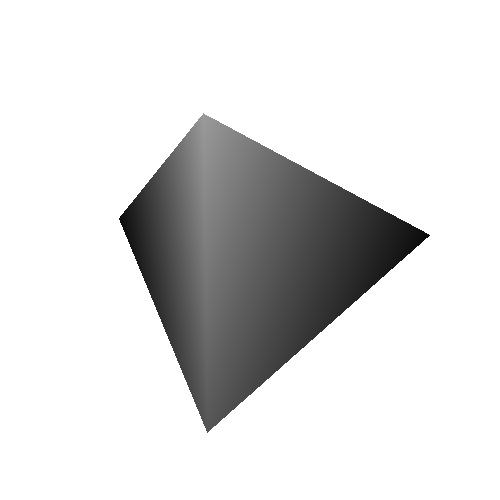
\includegraphics[scale=0.23]{../../Homework/3/data/hw3-4-a.png}\\
		{\small (a) \; 正四面体}
	\end{minipage}
	\begin{minipage}[b]{0.32\textwidth}
		\centering
		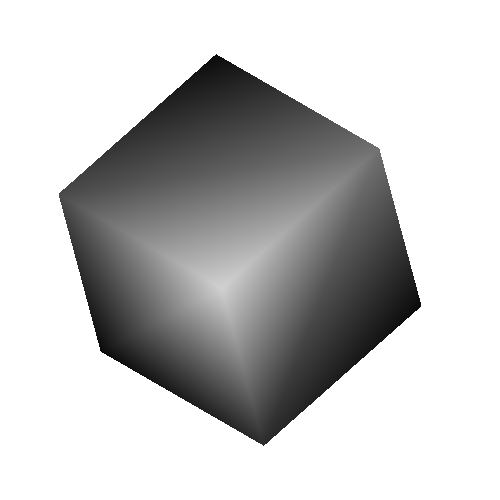
\includegraphics[scale=0.23]{../../Homework/3/data/hw3-4-b.png}\\
		{\small (b) \; 正六面体}
	\end{minipage}
	\begin{minipage}[b]{0.32\textwidth}
		\centering
		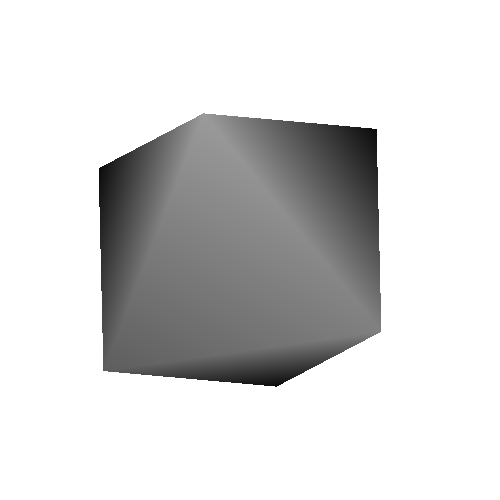
\includegraphics[scale=0.23]{../../Homework/3/data/hw3-4-c.png}\\
		{\small (c) \; 正八面体}
	\end{minipage}
	\caption{スムーズシェーディングで表示された正多面体}
	\label{fig:hw3-4}
\end{figure}

%%%%%%%%%%%%%%%%%%%%%%%%%%%%%%%%
%%% III-5
%%%%%%%%%%%%%%%%%%%%%%%%%%%%%%%%

\question{
	テキストのリスト27を参考に,アームロボットをシェーディング表示
	するものに変更してみよ.
}

% 文章

各パーツの角度を格納する\texttt{g\_rotAng}をグローバル変数に定義する.
そして各パーツを描画する前に関数\texttt{glRotated}を用いて回転させる.
\texttt{g\_rotAng}の値を書き換えるために\Lstref{lst:hw2-3-2}のキーボードコールバック関数を用いた.
ソースコードの他の部分はテキストのリスト27と同様である.
描画されたアームロボットを\Figref{fig:hw3-5}に示す.

\lstinputlisting[
	caption = アームロボットをシェーディング表示するプログラム(主要部),
	label = lst:hw3-5,
	linerange = {35-35, 44-50, 52-53, 55-57, 59-61, 63-64}
]{
	../../Homework/3/hw3-5.c
}

\begin{figure}[htbp]
	\centering
	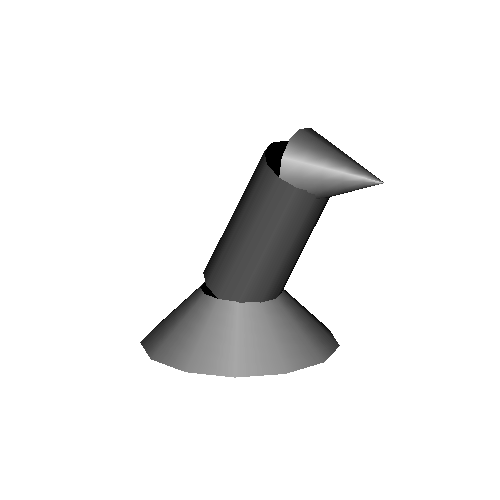
\includegraphics[scale=0.3]{../../Homework/3/data/hw3-5.png}\\
	\caption{シェーディング表示されたアームロボット}
	\label{fig:hw3-5}
\end{figure}
